\documentclass[conference]{IEEEtran}
\IEEEoverridecommandlockouts
\usepackage{inputenc}[utf8]
\usepackage[brazil]{babel}
\usepackage{cite}
\usepackage{amsmath,amssymb,amsfonts}
\usepackage{algorithmic}
\usepackage{graphicx}
\usepackage{textcomp}
\usepackage{xcolor}
\usepackage{fancyhdr}

\def\BibTeX{{\rm B\kern-.05em{\sc i\kern-.025em b}\kern-.08em
    T\kern-.1667em\lower.7ex\hbox{E}\kern-.125emX}}

\begin{document}
\title{Relatório de Modulação AM}

\author{
\IEEEauthorblockN{Luiz Felipe Rodrigues e Silva}
\IEEEauthorblockA{
\textit{Universidade de Brasília} \\
Brasília-DF, Brasil \\
luizrodriguesesilva@outlook.com.br}
}

\maketitle

\fancyhead{}
\fancyhead[L]{Relatório de Modulação AM}

\begin{abstract}
Este trabalho aborda a modulação em amplitude (AM), uma técnica clássica de transmissão de sinais analógicos, e suas variantes: AM convencional e AM com portadora suprimida (SC). São realizados dois experimentos utilizando o GNU Radio, nos quais são implementados e analisados tanto a modulação quanto a demodulação de sinais em ambas as técnicas. O objetivo é compreender, na prática, os conceitos teóricos estudados sobre modulação AM, observando as diferenças de desempenho e características entre os métodos, bem como os desafios envolvidos no processo de demodulação.
\end{abstract}

\begin{IEEEkeywords}
component, formatting, style, styling, insert.
\end{IEEEkeywords}

\section{Introdução}

A modução é um tecnica que permite a transmissão de sinais analógicos ou digitais através de um meio físico, como o ar ou cabos.
Segundo \cite{b12}, a modulação AM é um processo que envolve a variação da amplitude de uma portadora de alta frequência em função de um sinal modulante, que contém a informação a ser transmitida. Essa técnica é amplamente utilizada em sistemas de comunicação, como rádio e televisão, devido à sua simplicidade e eficácia na transmissão de sinais analógicos.


\subsection{Modulação AM-DSB-SC (Double Sideband Suppressed Carrier)}
A modulação AM-DSB (Double Sideband) é uma forma de modulação em que a portadora e as duas laterais (superior e inferior) são transmitidas. Esse tipo de modulação consiste em multiplicar o sinal de informação por uma portadora, como o sinal mensagem é de banda limitada, isto é, se o sinal $m(t)$ admite transformada de fourier, então $M(f) = 0$ para $|f| > W$, onde $W$ é a largura de banda do sinal.
Como a mensagem tem sua representação espectral, é possivel deslocar a mensagem para uma nova frequência utilizando a propriedade de modulação da transformada de Fourier, que nos diz que a multiplicação no domínio do tempo por uma exponencial complexa resulta em um deslocamento espectral no domínio da frequência. Multplicando o sinal de informação $m(t)$ por uma portadora $c(t) = A_{c} \cos(2 \pi f_{c} t)$, temos:
\begin{equation}
    s(t) = m(t) c(t) = A_{c} m(t) \cos(2 \pi f_{c} t)
\end{equation}

onde $A_{c}$ é a amplitude da portadora e $f_{c}$ é a frequência da portadora. Podemos expandir a expressão acima utilizando a identidade trigonométrica $\cos(x) = \frac{e^{jx} + e^{-jx}}{2}$, resultando em:

\begin{equation}
    s(t) = \frac{A_{c}}{2} m(t) e^{j 2 \pi f_{c} t} + \frac{A_{c}}{2} m(t) e^{-j 2 \pi f_{c} t}
\end{equation}

pode-se aplicar a transformada de Fourier em ambos os lados da equação, resultando em:

\begin{equation}
    S(f) = \frac{A_{c}}{2} (M(f - f_{c}) + M(f + f_{c}))
\end{equation}
Por exemplo, para uma mensagem $\cos(2\pi f_{m} t)$ com frequência $f_{m} = 100\,\text{Hz}$, uma portadora $\cos(2\pi f_{c} t)$ de $f_{c} = 1\,\text{kHz}$ com amplitude $A_{c} = 1$, realizando a modulação AM-DSB, os espectros para a mensagem, portadora e sinal modulado são mostrados nas Figuras~\ref{fig:espectro_mensagem}, \ref{fig:espectro_portadora} e \ref{fig:espectro_modulado}, respectivamente. O espectro do sinal modulado AM-DSB apresenta duas bandas laterais, uma superior e outra inferior, que contêm a mesma informação, além da portadora.

\begin{figure}[h]
    \centering
    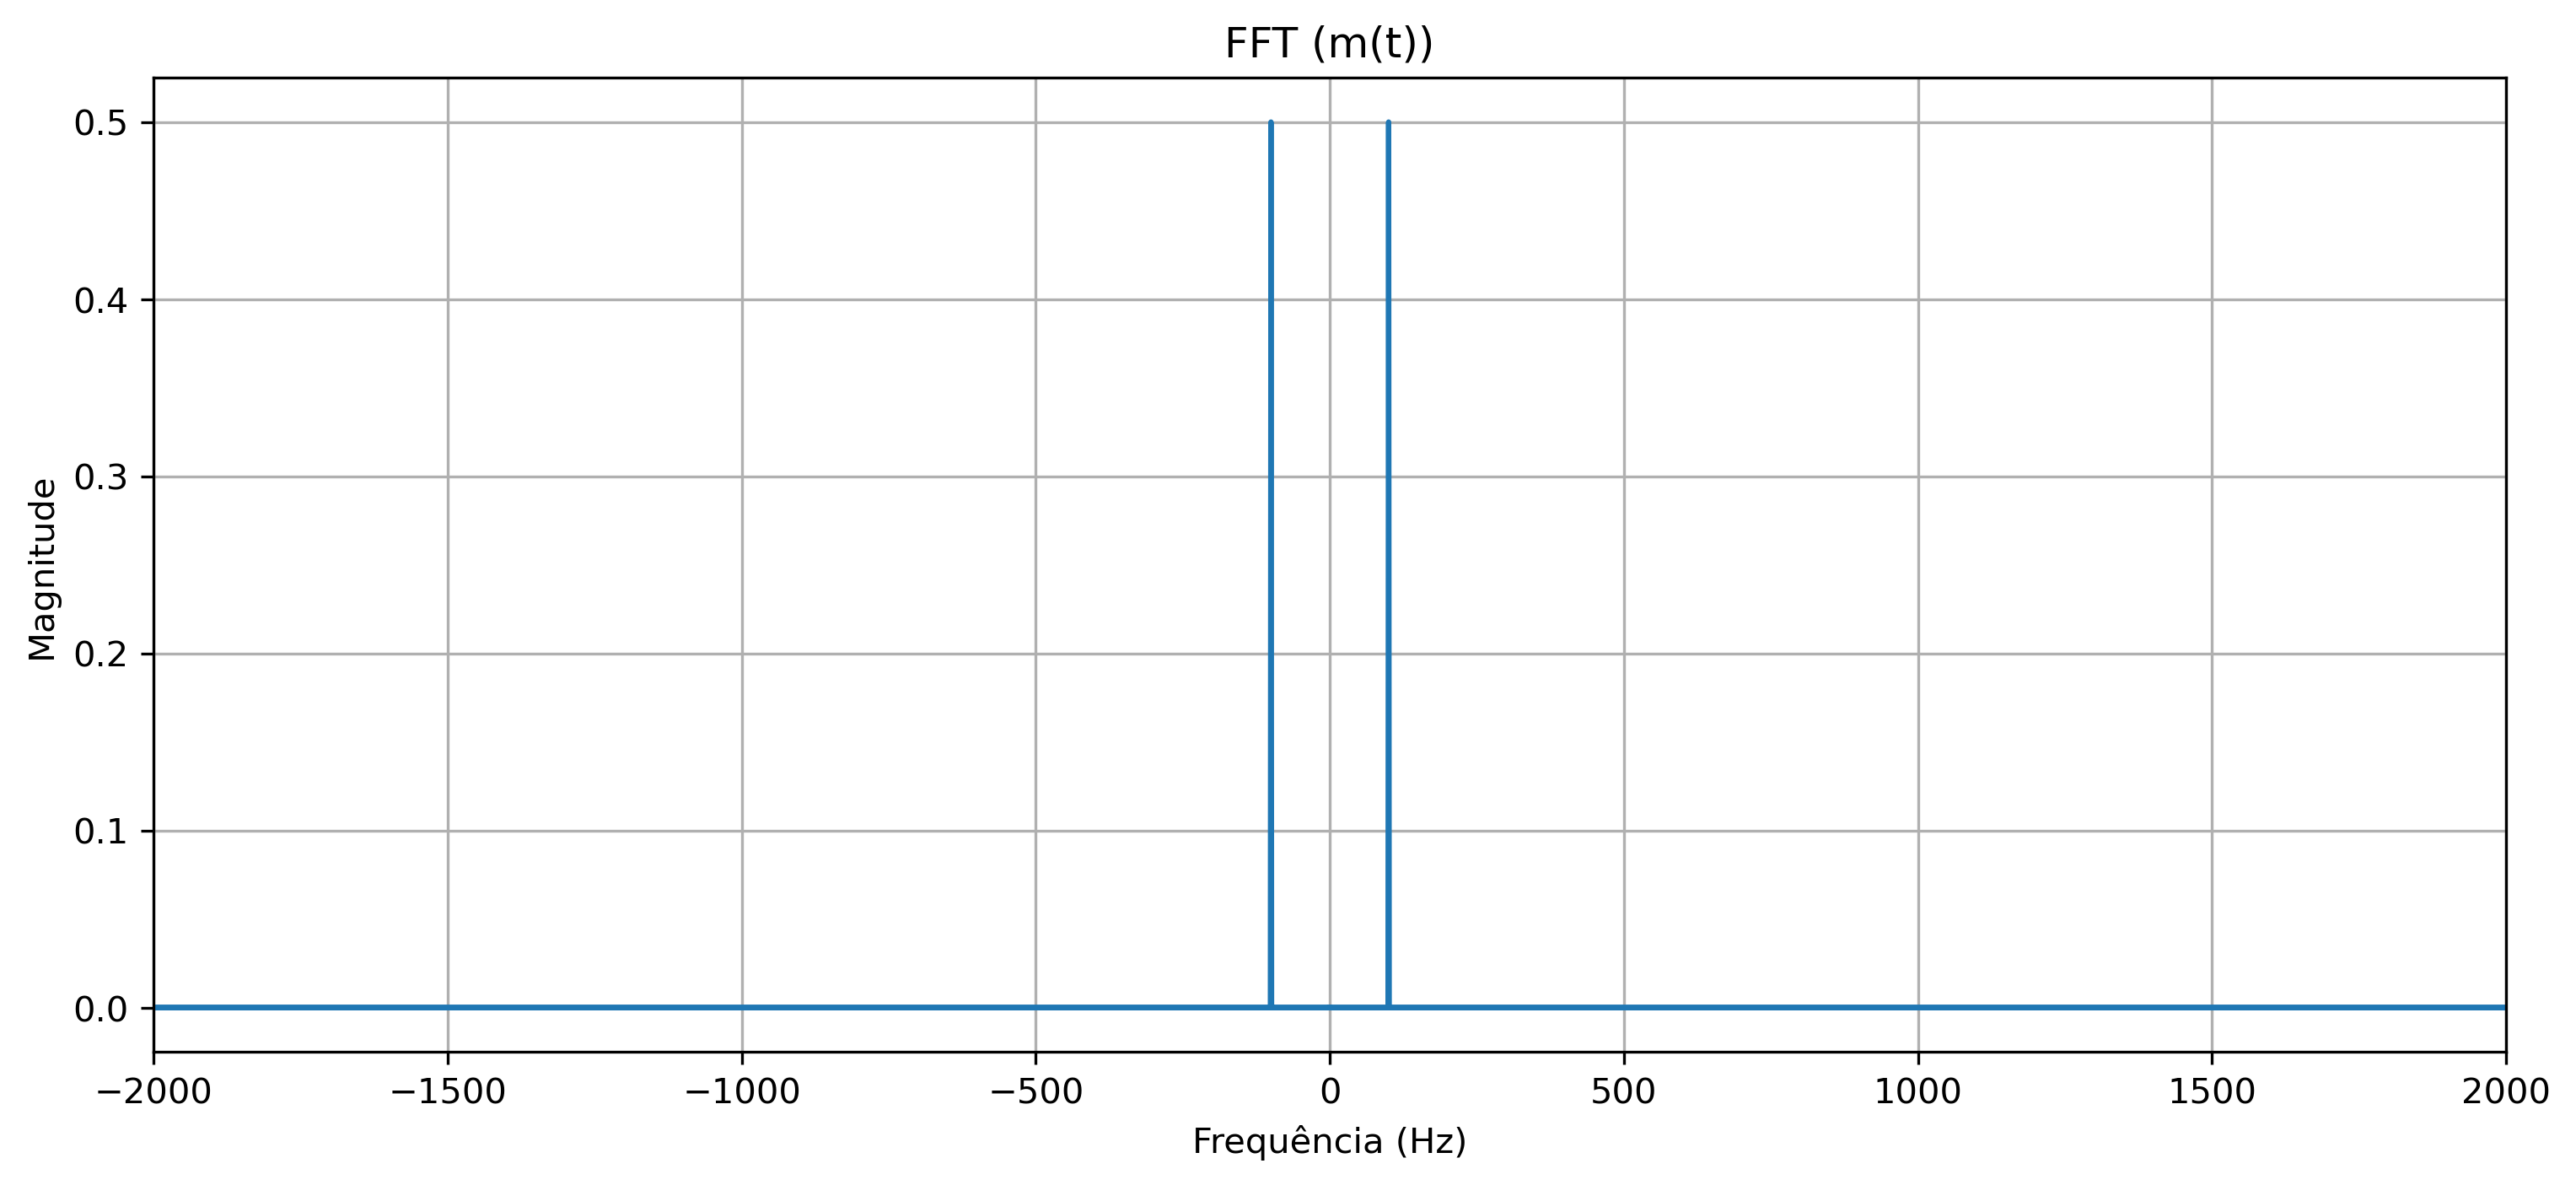
\includegraphics[width=0.5\textwidth]{images/FFT (m(t))_full.png}
    \caption{Espectro do sinal de mensagem. Fonte: Autor.}
    \label{fig:espectro_mensagem}
    \centering
\end{figure}

\begin{figure}[h]
    \centering
    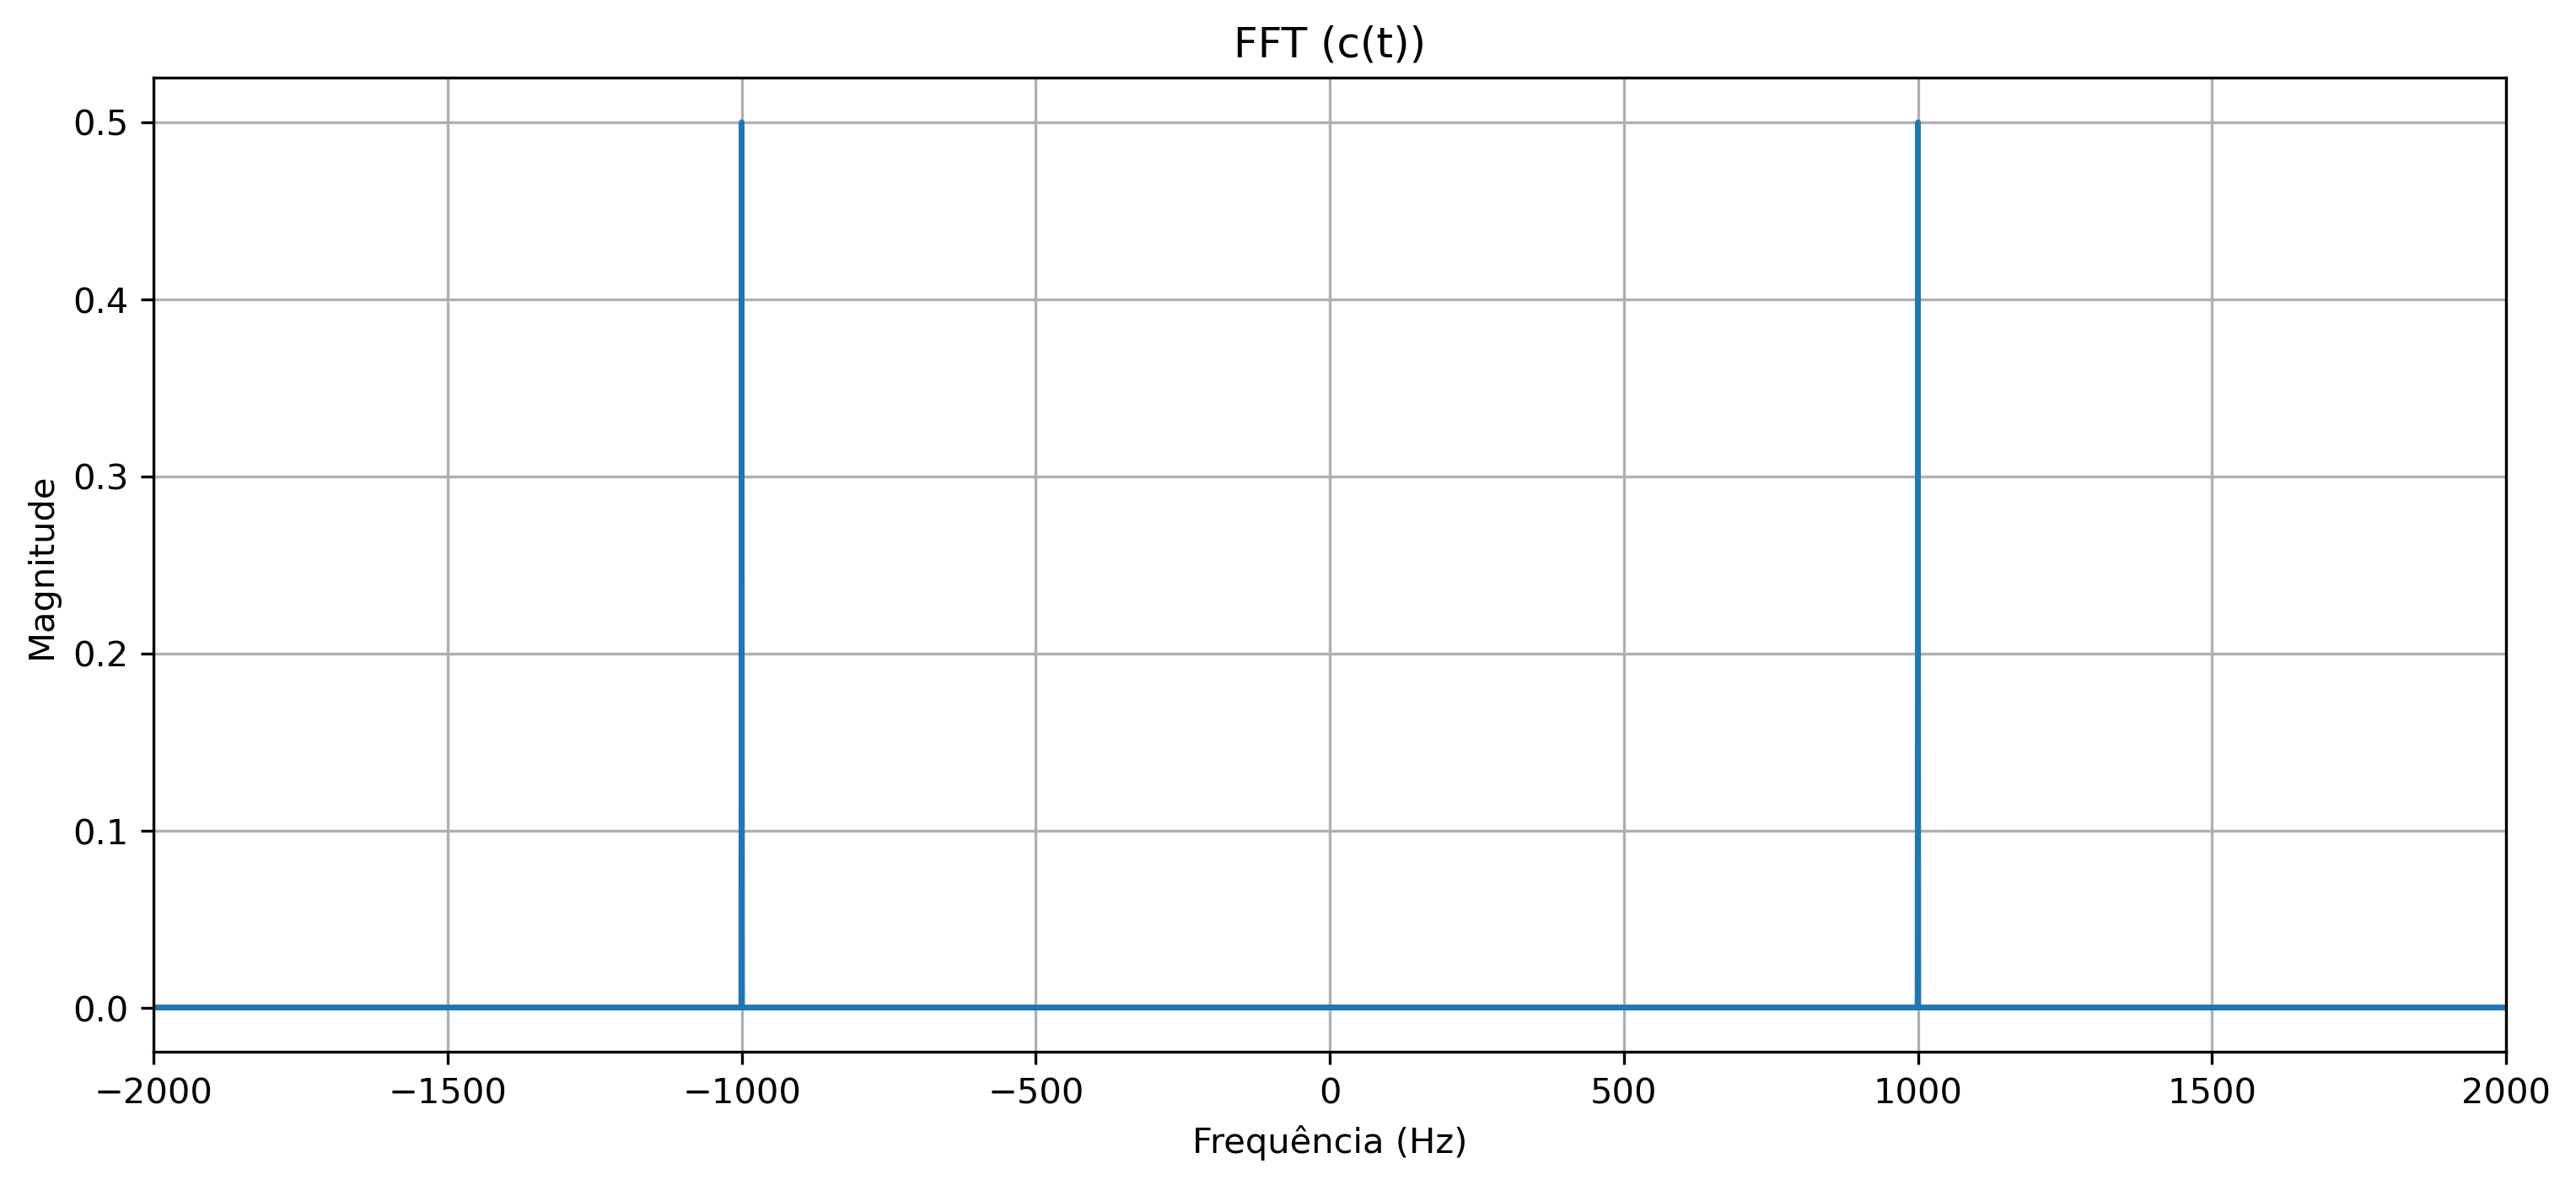
\includegraphics[width=0.5\textwidth]{images/FFT (c(t))_full.png}
    \caption{Espectro da portadora. Fonte: Autor.}
    \label{fig:espectro_portadora}
    \centering
\end{figure}

\begin{figure}[h]
    \centering
    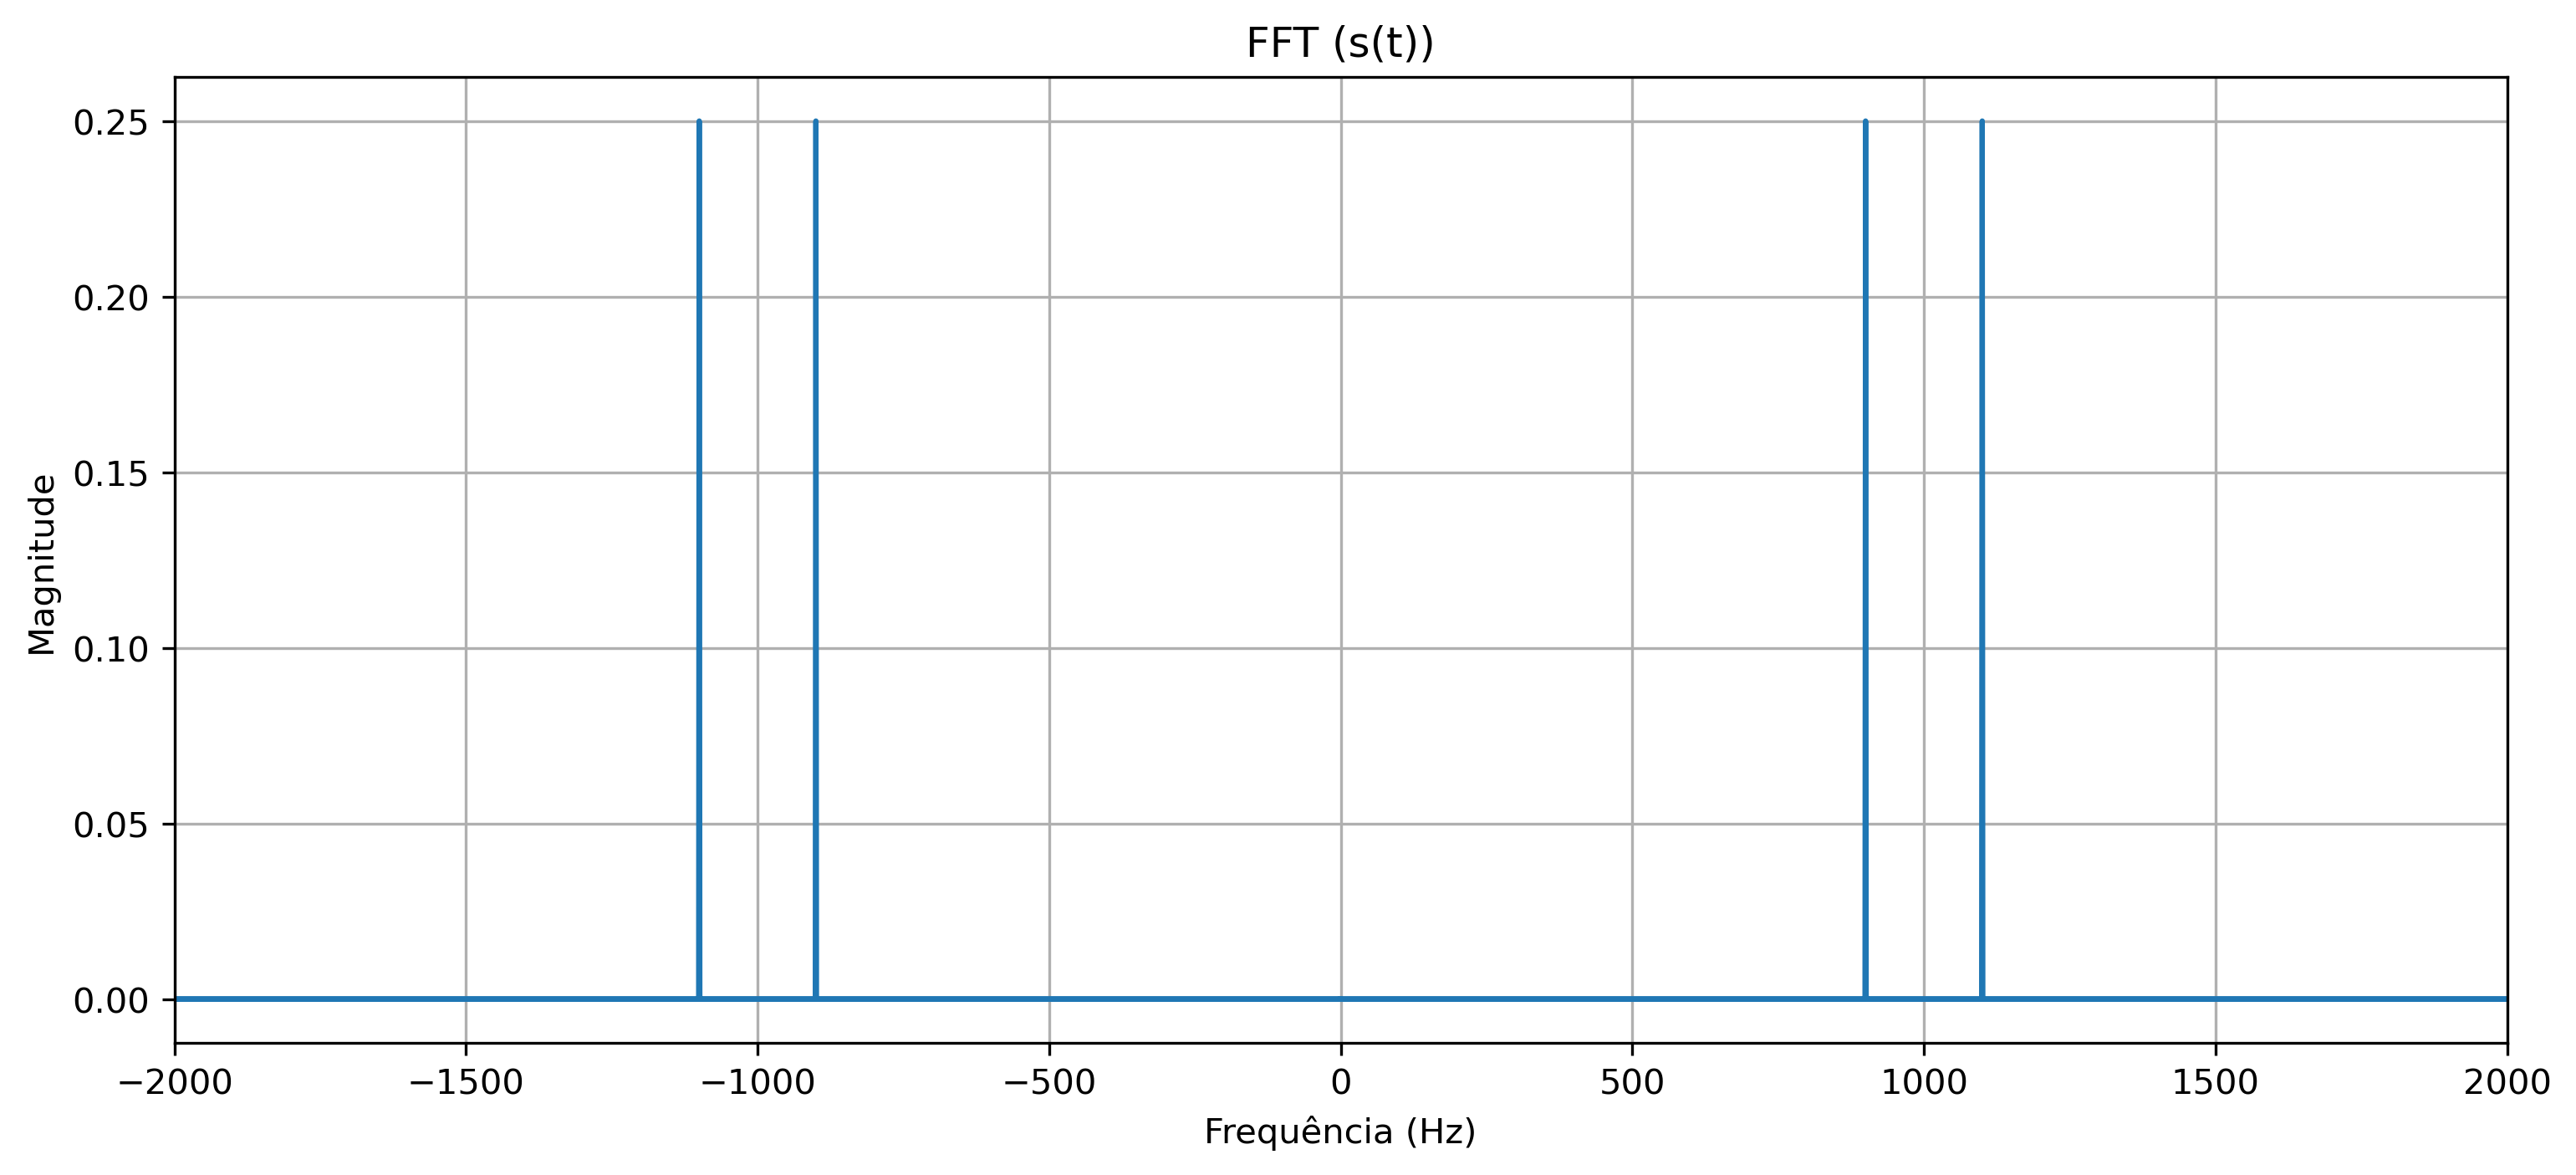
\includegraphics[width=0.5\textwidth]{images/FFT (s(t))_full.png}
    \caption{Espectro do sinal modulado AM-DSB. Fonte: Autor.}
    \label{fig:espectro_modulado}
    \centering
\end{figure}


O diagrama de blocos da modulação AM-DSB é apresentado na Figura \ref{fig:modulacao_am}, onde o sinal de informação $m(t)$ é multiplicado pela portadora $c(t)$, resultando no sinal modulado $s(t)$. A demodulação do sinal AM-DSB pode ser realizada utilizando um detector de envoltória, que recupera o sinal de informação original a partir do sinal modulado.

\begin{figure}[h]
    \centering
    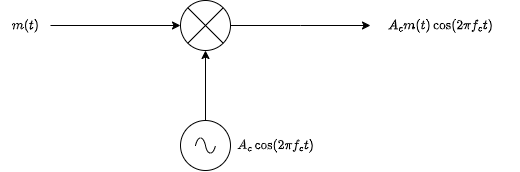
\includegraphics[width=0.5\textwidth]{images/modulacao_am.png}
    \caption{Diagrama de blocos da modulação AM-DSB. Fonte: Autor.}
    \label{fig:modulacao_am}
\end{figure}


Podemos demostrar os resultados a partir da transformada de Fourier, onde a transformada de Fourier do sinal modulado $m(t)$ é dada por:

\begin{equation}
    M(f) = \frac{1}{2} \left( \delta (f - 100) + \delta (f + 100) \right)
\end{equation}

substituindo na equação (3), temos:

\begin{align}
    S(f) = \frac{1}{4} \big(
        &\ \delta (f - 100 - 1000) + \delta (f + 100 - 1000) \notag \\
        &+ \delta (f - 100 + 1000) + \delta (f + 100 + 1000)
    \big)
\end{align}

Conforme mostrado no espectro \ref{fig:espectro_modulado}, a portadora é suprimida.


\subsection{demodulação AM-DSB-SC (Double Sideband Suppressed Carrier)}

A demodulação AM-DSB-SC é um processo que visa recuperar o sinal de informação original a partir do sinal modulado. O método mais comum para realizar essa demodulação é o uso de um multiplicador, que multiplica o sinal modulado por uma cópia da portadora. Esse processo resulta em um sinal que contém a informação original, mas também inclui uma componente de alta frequência que deve ser filtrada.

\begin{equation}
    s(t) = m(t) c(t) = A_{c} m(t) \cos(2 \pi f_{c} t)
\end{equation}

\begin{equation}
    y(t) = s(t) c(t) \cos(2 \pi f_{c}t)= A_{c} m(t) \cos(2 \pi f_{c} t)^{2}
\end{equation}

Linarizando o coseno, tempos:

\begin{equation}
    r(t) = \frac{A_{c}}{2} m(t) + \frac{A_{c}}{2} m(t) \cos(4 \pi f_{c} t)
\end{equation}

A transformada de Fourier do sinal demodulado $r(t)$ é dada por:

\begin{equation}
    Y(f) = \frac{A_{c}}{2} M(f) + \frac{A_{c}}{2} M(f - 2 f_{c}) + \frac{A_{c}}{2} M(f + 2 f_{c})
\end{equation}

Aplicando um filtro passa-baixa com largura de banda $W$ para eliminar a componente de alta frequência, obtemos o sinal de informação original:

\begin{equation}
    Y_{LPF}(f) = \frac{A_{c}}{2} M(f)
\end{equation}

O sinal é recuperado com uma amplitude reduzida, o que pode ser compensado por um amplificador. O diagrama de blocos da demodulação AM-DSB-SC é apresentado na Figura \ref{fig:demodulacao_am}, onde o sinal modulado $s(t)$ é multiplicado pela portadora $c(t)$, resultando no sinal demodulado $r(t)$. Em seguida, um filtro passa-baixa é aplicado para recuperar o sinal de informação original.

\begin{figure}[h]
    \centering
    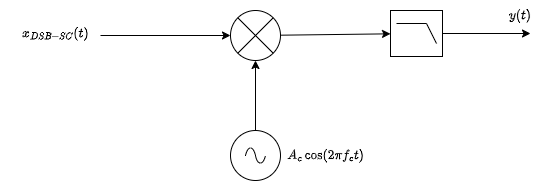
\includegraphics[width=0.5\textwidth]{images/demodulacao_am.png}
    \caption{Diagrama de blocos da demodulação AM-DSB-SC. Fonte: Autor.}
    \label{fig:demodulacao_am}
\end{figure}

Um dos principais desafios da modulação em amplitude com portadora suprimida (DSB-SC) é a necessidade de sincronização de fase entre o sinal modulado e a portadora na demodulação. Caso haja um desvio de fase entre a portadora original e a gerada no receptor, o sinal demodulado apresentará distorções significativas. Para mitigar esse problema, uma abordagem comum é transmitir um tom piloto juntamente com o sinal modulado. Esse tom é uma pequena fração da portadora original, inserida com baixa amplitude, e pode ser isolado no receptor por meio de um filtro de banda estreita. No entanto, a presença do tom piloto implica que a portadora não está totalmente suprimida, o que descaracteriza a modulação como DSB-SC pura.

Outra alternativa mais robusta é o uso de um PLL (Phase-Locked Loop), um circuito que sincroniza automaticamente a fase da portadora local com a fase do sinal modulado recebido. O PLL ajusta continuamente a frequência e a fase do oscilador local, permitindo uma demodulação mais precisa mesmo na presença de ruídos e desvios de fase. A Figura \ref{fig:demodulacao_am_pll} ilustra o esquema de demodulação utilizando PLL.

\begin{figure}[h]
    \centering
    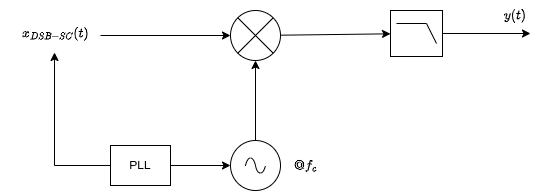
\includegraphics[width=0.5\textwidth]{images/demodulacao_am_pll.png}
    \caption{Diagrama de blocos da demodulação AM-DSB-SC com PLL. Fonte: Autor.}
    \label{fig:demodulacao_am_pll}
    \centering
\end{figure}

\subsection{Modulação AM Convencional}

Um sinal AM convencional consiste em uma componente portadora de grande amplitude, além do sinal modulado em DSB-AM. O sinal transmitido pode ser expresso matematicamente como:

\begin{equation}
u(t) = A_c[1 + m(t)] \cos(2\pi f_c t)
\end{equation}

onde $m(t)$ representa o sinal mensagem, o qual deve satisfazer a condição $|m(t)| \leq 1$ para garantir que a envoltória do sinal modulado permaneça sempre positiva. A componente $A_c m(t) \cos(2\pi f_c t)$ constitui o sinal DSB-AM, enquanto $A_c \cos(2\pi f_c t)$ representa a portadora.

A Figura~\ref{fig:am_envoltoria} ilustra a envoltória do sinal modulado:

\begin{figure}[h]
    \centering
    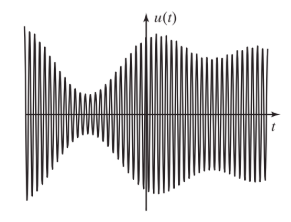
\includegraphics[width=0.3\textwidth]{images/envoltoria.png}
    \caption{Envoltoria do Sinal AM. Fonte: Proakis}
    \label{fig:am_envoltoria}
    \centering
\end{figure}

Na prática, o sinal $m(t)$ é escalado para garantir que sua magnitude esteja sempre dentro do intervalo desejado. Uma forma conveniente de fazer isso é expressar:

\begin{equation}
m(t) = a m_n(t)
\end{equation}

em que $m_n(t)$ é o sinal normalizado tal que seu valor mínimo é $-1$, definido por:

\begin{equation}
m_n(t) = \frac{m(t)}{\max |m(t)|}
\end{equation}

Nesse caso, o fator de escala $a$ é chamado de índice de modulação, sendo um valor constante geralmente menor que 1. Como $|m_n(t)| \leq 1$ e $0 < a < 1$, tem-se que $1 + a m_n(t) > 0$, evitando sobremodulação. Assim, o sinal modulado pode ser reescrito como:

\begin{equation}
u(t) = A_c[1 + a m_n(t)] \cos(2\pi f_c t)
\end{equation}

\subsubsection*{Espectro do Sinal AM Convencional}

Se $m(t)$ possui transformada de Fourier $M(f)$, o espectro do sinal modulado $u(t)$ será:

\begin{equation}
U(f) = \mathcal{F}\{A_c a m_n(t) \cos(2\pi f_c t)\} + \mathcal{F}\{A_c \cos(2\pi f_c t)\}
\end{equation}

\begin{equation}
U(f) = \frac{A_c a}{2}[M_n(f - f_c) + M_n(f + f_c)] + \frac{A_c}{2}[\delta(f - f_c) + \delta(f + f_c)]
\end{equation}

Portanto, o espectro de um sinal AM convencional ocupa uma largura de banda que é o dobro da largura de banda do sinal mensagem. A Figura \ref{fig:am_espectro}  apresenta o espectro $M(f)$.

\begin{figure}[h]
\centering
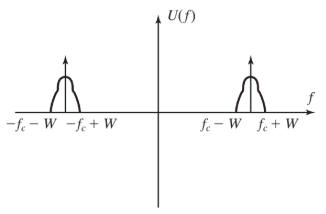
\includegraphics[width=0.3\textwidth]{images/espectro_am.png}
\caption{Sinal AM convencional no domínio do tempo e da frequência. Fonte: Proakis} 
\label{fig:am_espectro}
\end{figure}

A geração de um sinal AM pode ser feita utilziando um gerador de onda quadrada e um filtro passa banda

\begin{figure}[h]
\centering
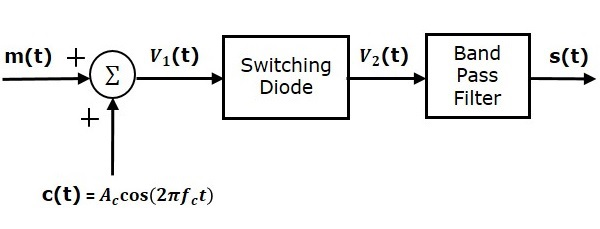
\includegraphics[width=0.3\textwidth]{images/blocos_amd_con.png}
\caption{Sinal no dominio da frequencia. Fonte: Tutorialspoint} 
\label{fig:diagrama_blocos_am_convencional}
\end{figure}

\subsection{demodulacao AM}

Existem diversas tencnias para demodular um sinal AM, neste trabalho iremos utilizar o detector de envoltoria. Basicamente
consiste em usar um circuito com um diodo e um filtro passa baixa.





\section{Metodologia}

O presente experimento foi desenvolvido com o objetivo de simular um sistema de modulação e demodulação em frequência (FM) utilizando o ambiente GNU Radio.

\subsection{Geração do Sinal FM}

A geração do sinal FM foi realizada a partir de um sinal senoidal com frequência de 1 kHz, representando o sinal de mensagem. Esse sinal foi conectado a um bloco \textbf{VCO (Voltage Controlled Oscillator)}, cuja frequência central foi configurada para 10 kHz.

O VCO gera um sinal cuja \textbf{frequência instantânea varia proporcionalmente à amplitude da senoide}, de acordo com a equação:

\begin{equation}
f_i(t) = f_c + k_f \cdot m(t)
\end{equation}

onde:
\begin{itemize}
    \item $f_i(t)$ = frequência instantânea;
    \item $f_c$ = frequência central da portadora (10 kHz);
    \item $k_f$ = sensibilidade de frequência do VCO, configurada como $2\pi \cdot f_c$;
    \item $m(t)$ = sinal de mensagem (senoide de 1 kHz).
\end{itemize}

Para permitir o ajuste dinâmico da amplitude do sinal de mensagem, foi utilizado um bloco \textbf{QT GUI Range}, com os seguintes parâmetros:
\begin{itemize}
    \item \textbf{Start}: 0
    \item \textbf{Stop}: 100 m
    \item \textbf{Step}: 2 m
    \item \textbf{Name}: amp
\end{itemize}

O controle da amplitude é fundamental, pois ela impacta diretamente no \textbf{desvio de frequência} ($\Delta f$) do sinal FM e, consequentemente, no \textbf{índice de modulação} ($\beta$), definido como:

\begin{equation}
\beta = \frac{\Delta f}{f_m}
\end{equation}

\noindent
sendo $f_m$ a frequência do sinal de mensagem (1 kHz).

Além disso, um bloco \textbf{Add Const} foi inserido com valor 1, garantindo que o sinal de entrada no VCO não assuma valores negativos, o que poderia causar deslocamentos indesejados na frequência portadora.

\begin{figure}[!h]
    \centering
    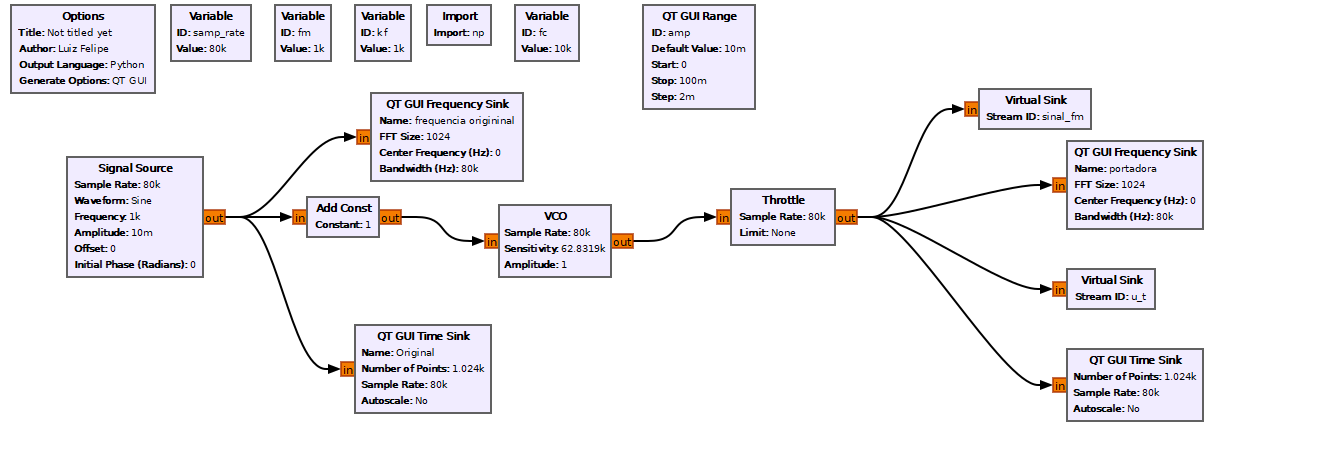
\includegraphics[width=0.5\textwidth]{images/FM_FLUXOGRAMA.png}
    \caption{Fluxograma do processo de modulação e demodulação FM.}
    \label{fig:fluxograma}
\end{figure}

\subsection{Demodulação do Sinal FM}

A recuperação do sinal de mensagem a partir do sinal FM foi realizada por meio da seguinte sequência de blocos:

\begin{enumerate}
    \item \textbf{Hilbert Transform}: o sinal real do VCO é convertido em um sinal complexo, gerando uma representação em banda unilateral. Este processo permite separar a informação de fase, necessária para demodulação baseada em frequência. O filtro de Hilbert foi configurado com \textbf{65 taps}, valor escolhido como compromisso entre resposta em frequência adequada e baixa distorção de fase, uma vez que um número maior de taps melhora a precisão, mas aumenta a latência.

    \item \textbf{Quadrature Demod}: esse bloco realiza a diferenciação da fase entre amostras consecutivas, estimando assim a \textbf{frequência instantânea}, proporcional ao sinal de mensagem. Sua operação é descrita matematicamente por:

    \begin{equation}
    y[n] = \frac{\mathrm{arg}\left( x[n] \cdot \overline{x[n-1]} \right)}{2\pi}
    \end{equation}

    O parâmetro de ganho foi configurado como:

    \begin{equation}
    \mathrm{Ganho} = \frac{\text{samp\_rate}}{2\pi \cdot f_c}
    \end{equation}

    Este fator de escala garante que o sinal demodulado corresponda numericamente à amplitude do sinal de mensagem, normalizando a saída de acordo com a frequência da portadora. Em termos práticos, esse ganho ajusta a sensibilidade do detector para converter variações de fase (em radianos) em variações proporcionais de frequência (em Hz) e, por consequência, em amplitude do sinal de mensagem.

    \item \textbf{Multiply Const}: etapa de ajuste fino na escala do sinal demodulado, permitindo calibrar a amplitude conforme desejado para comparação com o sinal original.

    \item \textbf{DC Block}: remove componentes de média (offset DC) que podem estar presentes após a demodulação. Esse offset geralmente é introduzido por imperfeições no processamento de fase e precisa ser removido para que o sinal tenha referência centrada em zero.

    \item \textbf{Filtro Passa-Baixa}: remove ruídos de alta frequência presentes na saída do quadrature demod, além de eliminar componentes residuais fora da banda do sinal de interesse. A configuração utilizada foi:
    \begin{itemize}
        \item \textbf{Frequência de corte}: 1.5 kHz, ligeiramente acima da frequência máxima do sinal de mensagem (1 kHz), garantindo a preservação total do conteúdo útil;
        \item \textbf{Largura de transição}: 500 Hz, proporcionando uma boa atenuação fora da banda sem exigir um filtro excessivamente complexo.
    \end{itemize}
\end{enumerate}

\begin{figure}[!h]
    \centering
    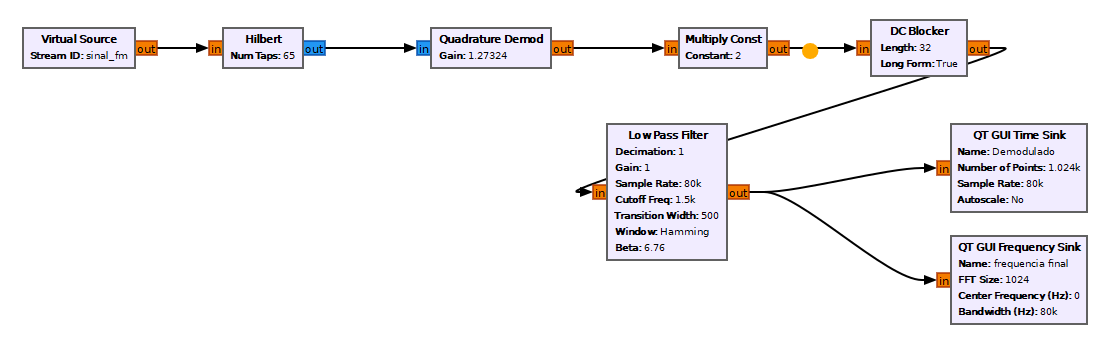
\includegraphics[width=0.5\textwidth]{images/DEM_FM.png}
    \caption{Diagrama de blocos da demodulação FM.}
    \label{fig:demodulacao}
\end{figure}


\subsection{Justificativa dos Parâmetros Escolhidos}

Os parâmetros foram definidos levando em consideração os seguintes critérios técnicos:

\begin{itemize}
    \item \textbf{Frequência de portadora (10 kHz)}: suficiente para separar a banda do sinal FM da baseband, permitindo uma representação clara da modulação.
    \item \textbf{Frequência de mensagem (1 kHz)}: escolhida para facilitar a visualização dos efeitos da modulação, estando confortavelmente abaixo da portadora.
    \item \textbf{Sensibilidade do VCO (2$\pi$ $\cdot$ 10k)}: essa escolha permite que a variação de fase no sinal FM corresponda diretamente à variação da amplitude do sinal de mensagem, alinhando os conceitos teóricos com a implementação prática.
    \item \textbf{Hilbert com 65 taps}: número suficiente para garantir boa precisão na conversão para sinal analítico sem exigir demasiada carga computacional.
    \item \textbf{Filtro passa-baixa com 1.5kHz}: protege contra aliasing e remove ruídos fora da banda, mantendo integralmente o conteúdo do sinal original.
\end{itemize}

\section{Experimentos}

\section{Resultados}

\subsection{Modulação AM-DSB-SC (Double Sideband Suppressed Carrier)}

Na modulação AM-DSB-SC, espera-se observar o espectro da mensagem deslocado para as frequências laterais em torno da frequência da portadora, conforme ilustrado na Figura~\ref{fig:sinais_freq_am_dsb}. Como pode ser visualizado, a mensagem original, que é uma senoide de 1~kHz, aparece como dois impulsos simétricos em torno da portadora de 5~kHz, definida pelo QT GUI Range. Isso ocorre devido à propriedade da modulação, que desloca o espectro da mensagem para as frequências $f_c + f_m$ e $f_c - f_m$, onde $f_c$ é a frequência da portadora e $f_m$ a frequência da mensagem.

\begin{figure}[h]
    \centering
    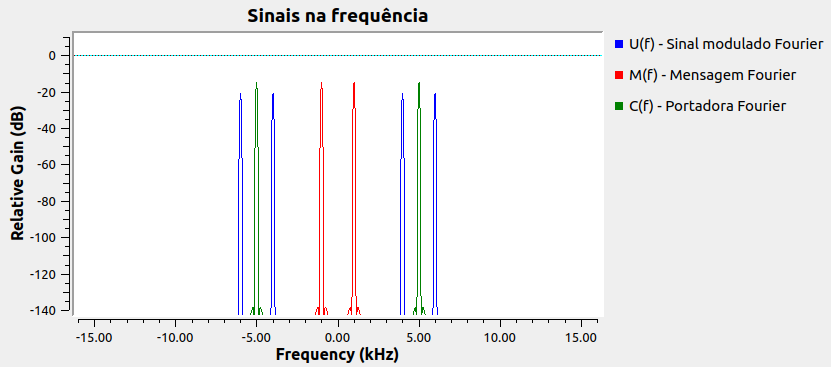
\includegraphics[width=0.5\textwidth]{images/sinais_freqe_gnu.png}
    \caption{Sinais no domínio da frequência. Fonte: Autor.}
    \label{fig:sinais_freq_am_dsb}
\end{figure}

\subsection{Demodulação AM-DSB-SC (Double Sideband Suppressed Carrier)}

Os resultados da demodulação também estão de acordo com o esperado. Ao utilizar um filtro passa-baixa com frequência de corte superior à largura de banda da mensagem, é possível recuperar o sinal original. A Figura~\ref{fig:demodulacao_am_dsb} mostra o espectro do sinal após a demodulação, evidenciando a recuperação da senoide de 1~kHz.

\begin{figure}[h]
    \centering
    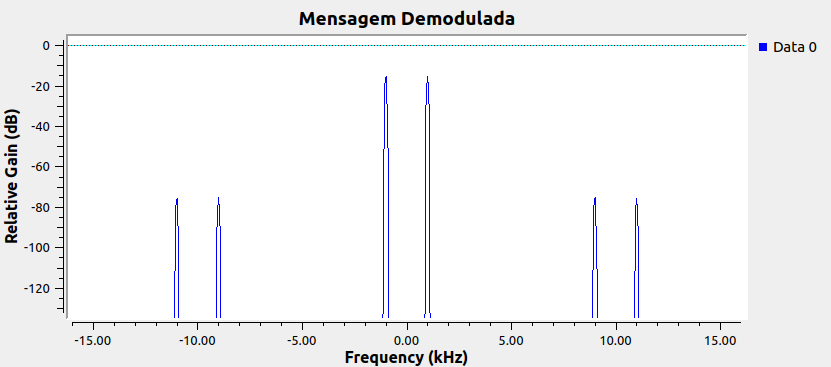
\includegraphics[width=0.5\textwidth]{images/demodulacao_am_dsb_freq.png}
    \caption{Demodulação do sinal AM-DSB-SC. Fonte: Autor.}
    \label{fig:demodulacao_am_dsb}
\end{figure}

\subsection{Falta de Sincronismo}

Para demonstrar que a demodulação AM-DSB-SC exige sincronismo entre a portadora do transmissor e do receptor, foi alterada a frequência da portadora local no receptor para 10~kHz utilizando o QT GUI Range, simulando uma perda de sincronismo de frequência. A Figura~\ref{fig:falta_sincronismo_dsb} mostra o espectro do sinal demodulado sob essa condição, evidenciando distorções e a impossibilidade de recuperar corretamente a mensagem original.

\begin{figure}[h]
    \centering
    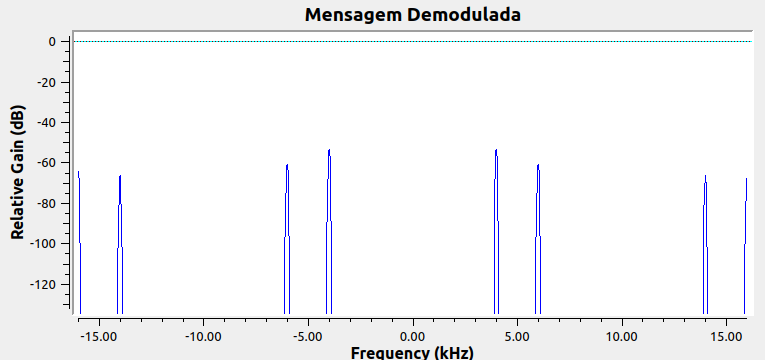
\includegraphics[width=0.5\textwidth]{images/falta_sincronismo_dsb.png}
    \caption{Simulação de falta de sincronismo na demodulação AM-DSB-SC. Fonte: Autor.}
    \label{fig:falta_sincronismo_dsb}
\end{figure}




\section{Discussão}


\begin{thebibliography}{00}
\bibitem{b12} NETO, Vicente S. Sistemas de Comunicação - Serviços, Modulação e Meios de Transmissão. Rio de Janeiro: Érica, 2015. E-book. p.44. ISBN 9788536522098. Disponível em: https://integrada.minhabiblioteca.com.br/reader/books/9788536522098/. Acesso em: 17 mai. 2025.
\bibitem{b13} Proakis, J. G., \& Salehi, M. (2005). Fundamentals of Communication Systems. McGraw-Hill.
\end{thebibliography}

\vspace{12pt}
\end{document}